\section{Аналитический раздел}

В данном разделе рассматривается задача распознавания образов. Рассматривается технология нейронных сетей, приводится обзор принципа работы нейронных сетей. Описываются виды нейронных сетей, их применение в задаче классификации. Дается обзор существующих методов распознавания образов на изображении.

\subsection{Задача распознавания образов}

Задачу распознавания образов (костей черепа лица и их повреждений в контексте работы) можно отнести к задаче классификации \cite{bones}. Классификация является одной из важнейших задач интеллектуального анализа данных. Она решается с помощью аналитических моделей, называемых классификаторами. Востребованность классификации обусловлена сравнительной простотой алгоритмов и методов ее реализации, и высокой интерпретируемостью результатов по сравнению с другими технологиями анализа данных.

В настоящее время разработано большое количество различных видов классификаторов, для построения которых используются как статистические методы (логистическая регрессия, дискриминантный анализ), так и методы машинного обучения (нейронные сети, деревья решений, метод k--ближайших соседей, машины опорных векторов) \cite{classifiers}.

Необходимость использования в анализе данных большого числа разнообразных методов классификации, обусловлена тем, что решаемые с ее помощью задачи могут иметь свои особенности, связанные, например, с числом классов (бинарная классификация или с несколькими классами) или с представлением исходных данных --- их объемом, размерностью и качеством, что требует выбора адекватного классификатора. Поэтому выбор классификатора, соответствующего особенностям решаемой задачи анализа, является важным фактором получения правильного решения \cite{choice}.

Различные виды классификаторов имеют свои преимущества и недостатки. Так, классификаторы, в которых используются методы статистики имеют хорошую математическую обоснованность, но при этом сложны в использовании и требуют знания вероятностного распределения исходных данных и оценки его параметров (поэтому их называют параметрическими), а также имеют фиксированную структуру модели. Кроме этого, статистические методы оценивают только вероятность принадлежности объекта классу, но не причину этой принадлежности.

Классификаторы, основанные на машинном обучении не требуют оценки параметров распределения исходных данных, а мера сходства в них формализуется с помощью функции расстояния (обычно, евклидова) \cite{euclidian}. Такие классификаторы называются метрическими. Как правило, они проще в реализации и использовании, чем параметрические, а их результаты удобнее для интерпретации и понимания. Но при этом метрические классификаторы являются эвристическими моделями --- обеспечивают решение только в ограниченном числе практически значимых случаев, могут дать неточное или не единственное решение. Поэтому использовать их результаты нужно с долей осторожности.

Определённым компромиссом между параметрическим и метрическими методами является использование для решении задач классификации нейронных сетей. Нейронные сети являются непараметрическими моделями, не требующими предположений о вероятностном распределении данных, но при этом и не используют меры расстояний. Это делает их универсальными классификаторами, позволяя получать результаты даже в случаях, когда параметрические и метрические классификаторы не обеспечиваю приемлемого решения.

\subsection{Нейронные сети}
\textit{Нейронные сети}, известные также как \textit{искусственные нейронные сети} или \textit{смоделированные нейронные сети}, являются подмножеством алгоритмов машинного обучения и служат основой для алгоритмов глубокого обучения. Понятие <<нейронные сети>> возникло при попытке смоделировать процессы, происходящие в человеческом мозге при передаче сигналов между биологическими нейронами \cite{neuralnet}.

Искусственные нейронные сети состоят из образующих слои узлов: слой входных данных, один или несколько скрытых слоев и слой выходных данных. Каждый узел (искусственный нейрон) связан с другими узлами с определенным весом и пороговым значением. Если вывод какого--либо узла превышает пороговое значение, то этот узел активируется и отправляет данные на следующий уровень сети. В противном случае данные на следующий уровень сети не передаются.

На рисунке \ref{fig:neuralnet} представлена модель работы нейронной сети, где $x_i$ --- входные данные, а $Y_j$ --- выходные данные.

\begin{figure}[H]
	\centering
	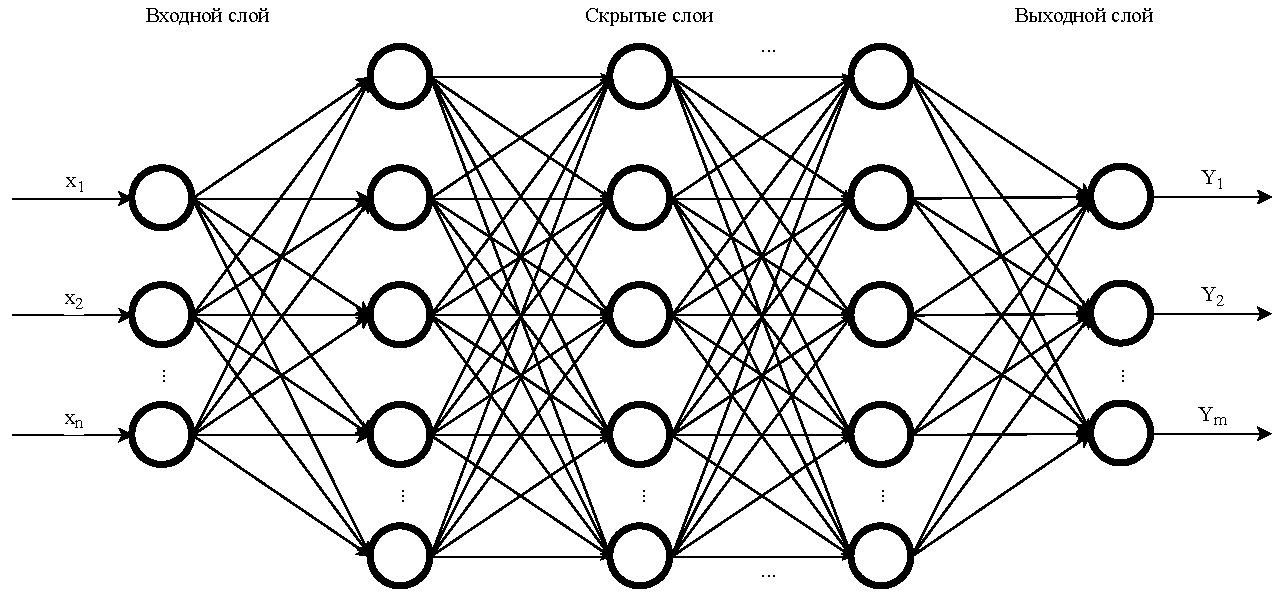
\includegraphics[width=\textwidth]{img/neuralnet.pdf}
	\caption{Модель нейронной сети}
	\label{fig:neuralnet}
\end{figure}

Для обучения и постепенного повышения точности нейронных сетей применяются обучающие данные. При достижении требуемой точности алгоритмы обучения превращаются в мощные инструменты для вычислений и искусственного интеллекта, что позволяет использовать их для классификации и кластеризации данных с высокой скоростью. Задачи из области распознавания речи или изображений можно выполнить за несколько минут, а не за несколько часов, как при распознавании вручную.

\subsubsection{Принцип работы нейронных сетей}

Каждый отдельный узел нейронной сети можно представить в виде модели линейной регрессии \cite{linearreg}, состоящей из входных данных, весовых коэффициентов, смещения (или порогового значения) и выходных данных. Эту модель можно описать следующей формулой:
\begin{equation}
	\label{eq:nn0}
	\hat{y} = \sum_{i=1}^{m}w_ix_i + bias
\end{equation}
\eqexplSetIntro{где}
\begin{eqexpl}[15mm]
\item{$m$} количество узлов нейронной сети;
\item{$w$} весовой коэффициент узла;
\item{$x$} единица входных данных;
\item{$bias$} значение ошибки.
\end{eqexpl}

Выходное значение для узла описывается по формуле:
\begin{equation}
	\label{eq:nn1}
	f(x_i) = \begin{cases}
		1 & \text{если $\sum_{i=1}^{m}w_ix_i + bias \ge 0$}\\
		0 & \text{иначе.}\\
		\end{cases}
\end{equation}

После определения слоя входных данных необходимо назначить весовые коэффициенты. Они помогают определить важность той или иной переменной: чем выше весовой коэффициент, тем существеннее его вклад в выходные данные по сравнению с другими входными данными. Затем произведения входных данных и соответствующих им весовых коэффициентов суммируются. Наконец, выходные данные передаются через функцию активации \ref{eq:nn1}, которая вычисляет результат. Если полученный результат превышает установленное пороговое значение, узел срабатывает (активируется), передавая данные на следующий слой сети. Выходные данные одного узла становятся входными данными для следующего узла. Такой последовательный процесс передачи данных между слоями характерен для нейронных сетей прямого распространения.

Для более наглядной демонстрации этой концепции рассмотрим реальный пример: допустим, нужно принять решение, стоит ли идти на серфинг (Да: 1, Нет: 0). Решение <<идти>> или <<не идти>> --- прогнозируемый результат $\hat{y}$. Предположим, существует три фактора, которые влияют на принятие решения:

\begin{enumerate}[leftmargin=1.6\parindent]
	\item Хорошие ли сегодня волны? (Да: 1, Нет: 0)
	\item Свободна ли зона для плавания? (Да: 1, Нет: 0)
	\item Были ли случаи нападения акул в последнее время? (Да: 0, Нет: 1)
\end{enumerate}

Предположим, что имеются следующие входные данные:

\begin{itemize}[leftmargin=1.6\parindent]
	\item $x_1 = 1$, так как сегодня хорошие волны для серфинга;
	\item $x_2 = 0$, так как уже собралось много серферов;
	\item $x_3 = 1$, так как в последнее время не было нападений акул.
\end{itemize}

Теперь нужно присвоить весовые коэффициенты для определения важности. Чем выше значение весового коэффициента, тем большим будет влияние конкретной переменной на решение или результат.

\begin{itemize}[leftmargin=1.6\parindent]
	\item $w_1 = 5$, так как большие волны --- редкость;
	\item $w_2 = 2$, так как скопление серферов не является проблемой;
	\item $w_3 = 4$, так как присутствует страх к акулам.
\end{itemize}

Приняв пороговое значение ($bias$) равным 3 (случайно выбранное значение для примера), можно подставить значения в формулу \ref{eq:nn0} и получить результат.

\begin{equation}
	\label{eq:nn2}
	\hat{y} = (1 * 5) + (0 * 2) + (1 * 4) - 3 = 6
\end{equation}

С помощью функции активации из формулы \ref{eq:nn1}, можно вычислить выходные данные для этого узла: результат равен 1, так как 6 больше 0. Это означает, что в примере стоит идти на серфинг; если же изменить весовые коэффициенты или пороговое значение, результат вычисления для данной модели может отличаться. 

Из примера следует, что нейронная сеть способна принимать решения с возрастающей степенью сложности, в зависимости от выходных данных предыдущих решений или слоев. Для иллюстрации математических понятий были использованы персептроны, в то время как в нейронных сетях применяются сигмоидальные нейроны, значения которых могут находиться в диапазоне от 0 до 1. По своему принципу работы нейронные сети схожи с деревьями принятия решений, поэтому в результате передачи данных от одного узла к другому, при $x$ значений от 0 до 1, влияние того или иного изменения отдельной переменной на выходные данные любого узла и, следовательно, выходные данные нейронной сети уменьшается.

В более практических сценариях использования нейронных сетей, например распознавание или классификация изображений, для обучения алгоритма используется контролируемое обучение или маркированные наборы данных. В ходе обучения модели потребуется оценить точность с помощью функции стоимости (среднеквадратическая ошибка). Функция стоимости выражается с помощью формулы:
\begin{equation}
	\label{eq:nn3}
	Cost Function = \frac{1}{2m}\sum_{i=1}^{m}(\hat{y}-y)^2
\end{equation}
\eqexplSetIntro{где}
\begin{eqexpl}[15mm]
	\item{$i$} индекс выборки;
	\item{$\hat{y}$} прогнозируемое значение;
	\item{$y$} фактическое значение;
	\item{$m$} число выборок.
\end{eqexpl}

Конечная цель --- минимизировать функцию стоимости, чтобы обеспечить корректность для каждого отдельно взятого наблюдения. В процессе корректировки весовых коэффициентов и смещения модель использует функцию стоимости и обучение с подкреплением для достижения точки сходимости или локального минимума. Корректировка весовых коэффициентов происходит с помощью алгоритма градиентного спуска, что позволяет определить стратегию уменьшения количества ошибок (или минимизации функции стоимости). С каждым шагом обучения параметры модели корректируются, пока не будет достигнут минимум. На рисунке \ref{fig:cost} изображен процесс минимизации функции стоимости.

\begin{figure}[H]
	\centering
	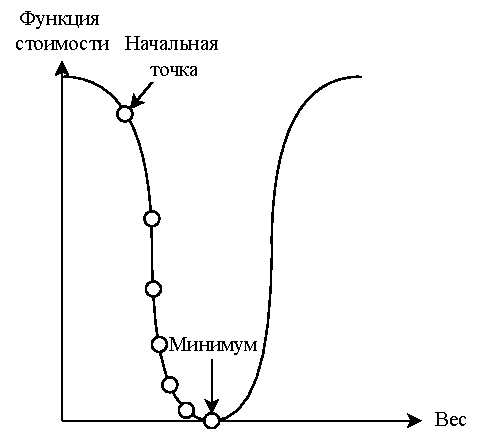
\includegraphics[width=\textwidth]{img/cost.pdf}
	\caption{Минимизация функции стоимости}
	\label{fig:cost}
\end{figure}

Большинство глубоких нейронных сетей относятся к алгоритмам прямого распространения, т. е. данные передаются только в одном направлении --- от входа к выходу. Однако для обучения моделей может также применяться метод обратного распространения ошибки, когда данные передаются в противоположном направлении --- от выхода к входу. Метод обратного распространения ошибки позволяет вычислить и объяснить ошибки, связанные с каждым нейроном, что позволяет скорректировать и адаптировать параметры модели соответствующим образом.

\subsubsection{Виды нейронных сетей}

Нейронные сети можно разделить на несколько видов, в зависимости от целевого назначения. 

\textit{Персептрон} --- первая нейронная сеть, созданная Фрэнком Розентблаттом в 1958 году. Она содержит один нейрон и представляет собой простейшую форму нейронной сети. На рисунке \ref{fig:perceptron} изображен пример такой нейронной сети.

\begin{figure}[H]
	\centering
	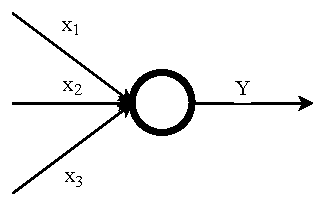
\includegraphics[width=\textwidth]{img/perceptron.pdf}
	\caption{Персептрон}
	\label{fig:perceptron}
\end{figure}

\textit{Нейронные сети прямого распространения (многослойные персептроны (MLP)} --- нейронные сети, состоящие из слоев входных данных, одного или нескольких скрытых слоев и выходных данных. Данные, поступающие в эти модели, используются для обучения. Эти сети лежат в основе алгоритмов компьютерного зрения, обработки данных на естественном языке и других нейронных сетей.

\textit{Рекуррентные нейронные сети (RNN)} имеют в своем составе обратные связи. Такие алгоритмы обучения используются в основном для временных рядов данных с целью прогнозирования будущих событий, например стоимости акций на фондовых биржах или объема продаж.

\subsubsection{Сравнение нейронных сетей и глубокого обучения}

Часто термины <<глубокое обучение>> и <<нейронные сети>> могут использоваться как синонимы, что не совсем верно. Стоит отметить, что понятие <<глубина>> в <<глубоком обучении>> характеризует лишь количество слоев нейронной сети. Нейронную сеть, в составе которой более трех слоев (включая слой входных данных и слой выходных данных), можно отнести к алгоритмам глубокого обучения. Нейронная сеть с двумя--тремя уровнями считается простой нейронной сетью.

\subsubsection{Особенности применения нейронных сетей в качестве классификаторов}

Задача классификации для нейронных сетей не является основной. Основной задачей для нейронных сетей является численное предсказание (как было показано на примере с серфингом).

Используя специальные способы представления данных, можно адаптировать нейронные сети для работы с категориальными данными, т.е. получать на вход и формировать на выходе категориальные значения. Для этого категориальные признаки соответствующим образом кодируются с помощью числовых значений.

Нейронные сети имеют ряд преимуществ при использовании в качестве классификаторов. Например:
\begin{itemize}[leftmargin=1.6\parindent]
	\item нейронные сети являются самообучаемыми моделями, работа которых практически не трубет вмешательства пользователя;
	\item нейронные сети являются универсальными аппроксиматорами, позволяющими аппроксимировать любую непрерывную функцию с приемлемой точностью;
	\item нейронные сети являются нелинейными моделями, что позволяет эффективно решать задачи классификации даже при отсутствии линейной разделимости классов. На рисунке \ref{fig:separation} приведен пример линейной разделимости и неразделимости классов.
\end{itemize}

\begin{figure}[H]
	\centering
	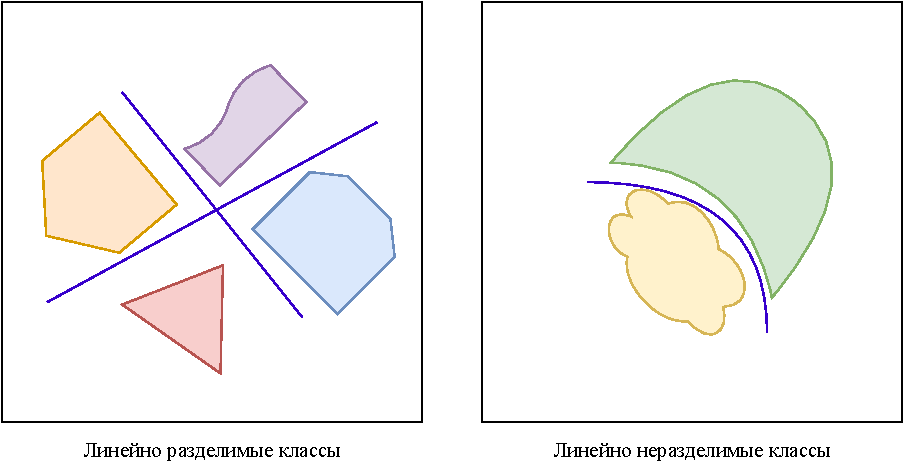
\includegraphics[width=\textwidth]{img/separation.pdf}
	\caption{Линейная разделимость классов}
	\label{fig:separation}
\end{figure}

Следует отметить, что каких--либо специальных нейросетевых архитектур для классификации не существует. Наиболее часто используемой для классификации архитектурой нейронных сетей являются сети прямого распространения, на входные нейроны которых подаются значения признаков классифицируемого объекта, а на выходе формируется метка или числовой код класса.

Последующие слои, таким образом, разделяют объекты на классы в пространстве признаков более высокой размерности, чем исходное. Например, если размерность вектора признаков исходных данных равна 4, и скрытый слой содержит 6 нейронов, то выходной слой производит разбиение объектов на классы в 6--мерном пространстве.

Это позволяет сделать процесс более эффективным: правильно подобрав конфигурацию и параметры нейронной сети, можно получить хорошие результаты классификации даже в тех случаях, когда классификаторы других типов, работающие только в размерности обучающих данных, не обеспечивают приемлемых результатов. Недостатком является то, что конфигурация сети, наилучшим образом аппроксимирующая функцию разделения классов в пространстве признаков, заранее неизвестна. Поэтому приходится подбирать её экспериментально, либо использовать опыт аналогичных решений.

Если распределение классов таково, что для их разделения требуется сложная функция, размерность нейронной сети может оказаться неприемлемо большой. В этом случае проблему можно решить с помощью специальной предобработки исходных данных.

\subsection{Методы и технологии распознавания образов}

Для решения задачи распознавания образов с помощью нейронных сетей применяются такие способы, как:
\begin{itemize}[leftmargin=1.6\parindent]
	\item R--CNN (от англ. Region--based Convolutional Network);
	\item Fast R--CNN;
	\item Faster R--CNN. 
\end{itemize}

\subsubsection{R--CNN}

R--CNN имеет следующую схему работы:
\begin{enumerate}[leftmargin=1.6\parindent]
	\item При помощи \textit{selective search} (с англ. избирательный поиск)  \cite{selsearch} на изображении выделяются регионы, которые предположительно содержат объект (кости лица на КТ или МРТ снимке).
	\item Регион--претендент при помощи аффинного преобразования отображается в квадрат 227$\times$227.
	\item Полученный прямоугольник подается на вход сети \cite{imagenet}, которая имеет структуру, представленную на рисунке \ref{fig:rcnn}.
	 \begin{figure}[H]
	 	\centering
	 	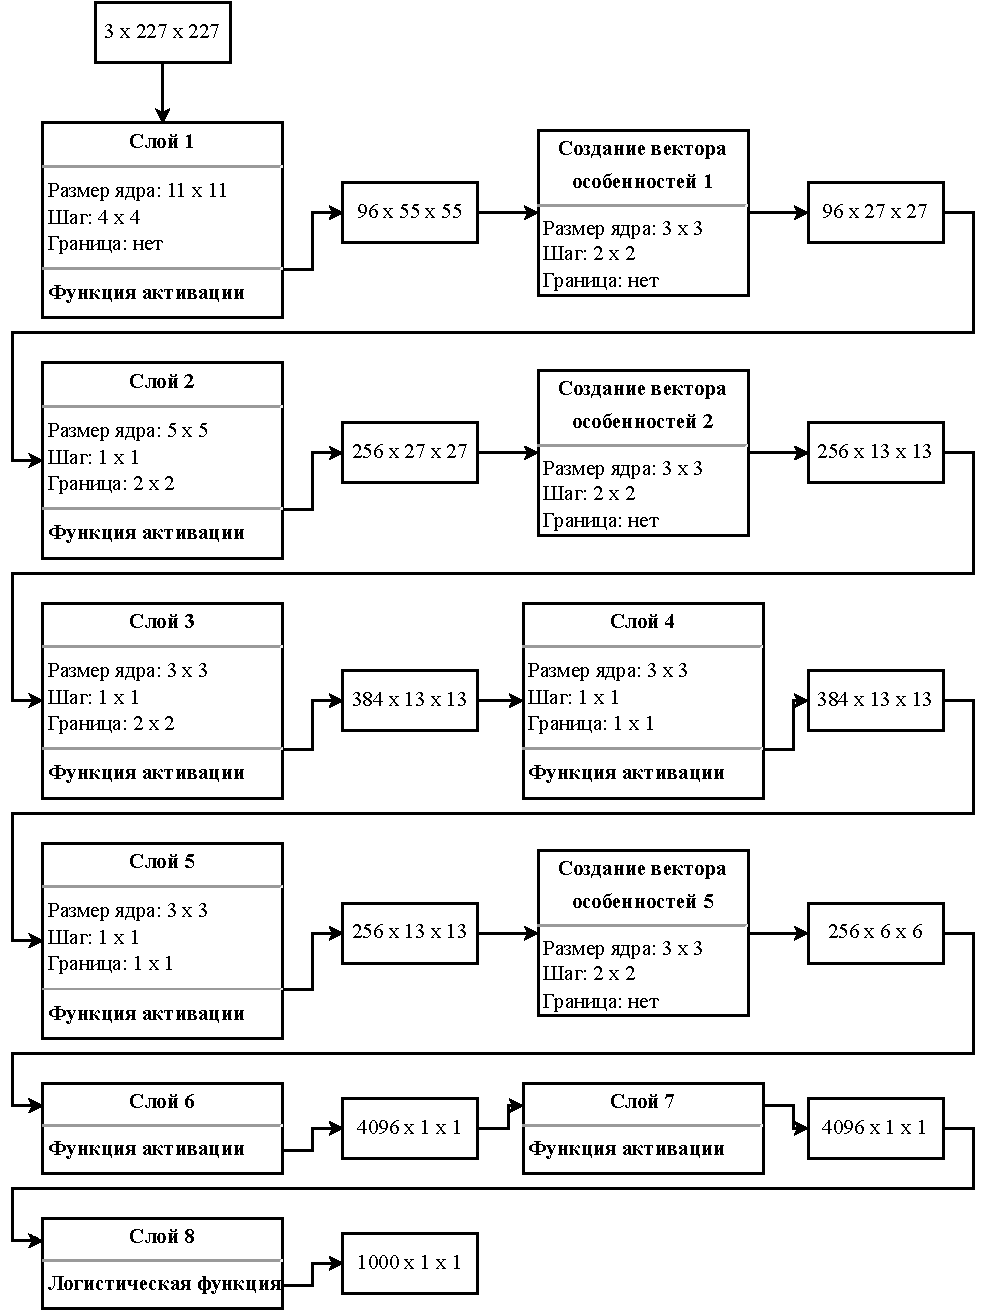
\includegraphics[width=\textwidth]{img/rcnn.pdf}
	 	\caption{Принцип работы R--CNN}
	 	\label{fig:rcnn}
	 \end{figure}
 	\item С седьмого слоя сети снимается вектор размерности 4096. Этот вектор используется в машине опорных векторов, натренированной для каждого класса, для классификации.
 	\item Вектор подается в линейный регрессор (логистическая функция), соответствующий классу объекта для восстановления позиции объекта.
\end{enumerate}

\subsubsection{Fast R--CNN}

R--CNN имеет несколько недостатков, в основном связанных с высокими временными затратами:
\begin{enumerate}[leftmargin=1.6\parindent]
	\item Требуется натренировать сверточную нейронную сеть (в два этапа: тренировка без точной разметки и оптимизация для 20 классов).
	\item Требуется натренировать набор машин опорных векторов по одной для каждого класса. При этом на вход машина опорных векторов принимает вектора особенностей, полученных от натренированной сверточной сети. Эти вектора нужно изначально вычислить на наборе данных, используемых для тренировки.
	\item Требуется натренировать линейные регрессоры (по одному для каждого класса) для восстановления позиций объекта.
	\item Процесс детектирования и классификации требует существенного времени (до 49 секунд на одно изображение) \cite{fastrcnn}.
\end{enumerate}

Существенные временные затраты на этапе детектирования сильно снижают практическую пользу R--CNN. Причина, из--за которой детектирование работает так медленно, заключается в том, что при помощи избирательного поиска генерируется примерно 2000 претендентов на изображении, и каждый претендент должен быть пропущен через сверточную сеть, чтобы вычислить для него вектор особенностей. Процесс этот достаточно затратный, особенно для сетей с большим числом сверточных слоев. В Fast R--CNN предлагают подавать на вход сети полное изображение, но при этом последний слой заменить на слой типа \textit{RoI pooling} (Region of Interest Pooling) \cite{fastrcnn}.

\textit{RoI pooling} слой принимает на вход карту особенностей, полученную от последнего сверточного слоя нейронной сети, и RoI претендента (в координатах изображения). RoI преобразуется из координат изображения в координаты на карте особенностей и на полученный прямоугольник накладывается сетка $W \times H$ с наперед задаными размерами (например, $W = H = 7$) \cite{fastrcnn}. RoI pooling слой преобразует вектор особенностей произвольного прямоугольника из исходного изображения в вектор особенностей фиксированной размерности.

После RoI pooling слоя данные через два полносвязных слоя подаются параллельно на слой для оценки принадлежности претендента одному из классов объектов и слой, реализующий регрессию для уточнения границы объекта.

Итоговый принцип работы Fast R--CNN представлен на рисунке \ref{fig:fastrcnn}.

\begin{figure}[H]
	\centering
	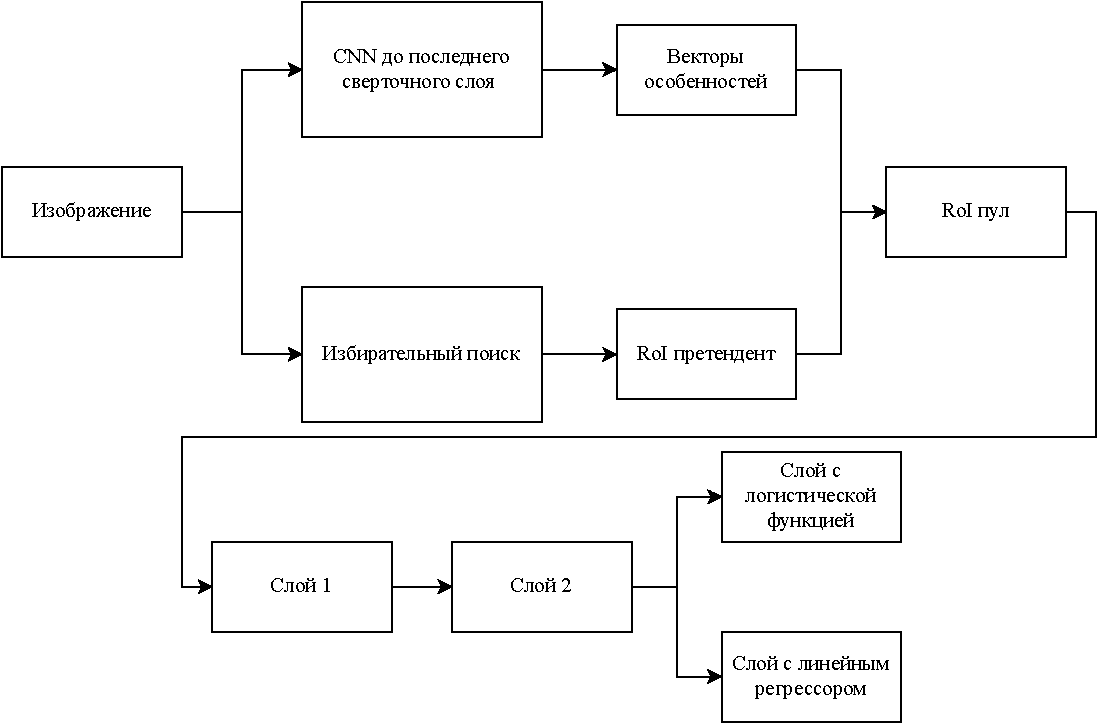
\includegraphics[width=\textwidth]{img/fastrcnn.pdf}
	\caption{Принцип работы Fast R--CNN}
	\label{fig:fastrcnn}
\end{figure}

В отличии от R--CNN, где карта особенностей генерировалась для каждого претендента на изображении, в Fast R--CNN генерируется карта особенностей для всего изображения, а затем при помощи специального слоя из нее вычленяются карты для каждого из претендентов, что позволяет существенно сократить время вывода.

\subsubsection{Faster R--CNN}

В качестве улучшения Fast R--CNN предлагается замена процедуры генерации претендентов избирательным поиском на нейронную сеть, которая использует имеющуюся карту особенностей (для примера, VGG16) \cite{fasterrcnn}. Для изображения размера $W_1 \times H_1$ на выходе последнего сверточного слоя сеть VGG16 выдает карту особенностей с размерами $W_1/16 \times H_1/16$, вектор особенностей для каждой точки будет иметь размерность 512. При этом вектор особенностей в точке ($x_f, y_f$) вносят вклад точки изображения, лежащие внутри квадрата с центром в ($16x_f, 16y_f$) и размера 196 $\times$ 196.

Для каждой точки карты особенностей ($x_f, y_f$) проверяется $k$ претендетов разных размеров на изображении в регионах с центром в ($16x_f, 16y_f$). Рассматривают 9 претендентов, варьируя три масштаба и три отношения сторон ($1\div1, 1\div2, 2\div1$). Для решения задачи используется \textit{Region Proposal Network (RPN)} (от англ. сеть для предложения регионов) \cite{rpn}.

Итоговый принцип работы Faster R--CNN представлен на рисунке \ref{fig:fasterrcnn}.

\begin{figure}[H]
	\centering
	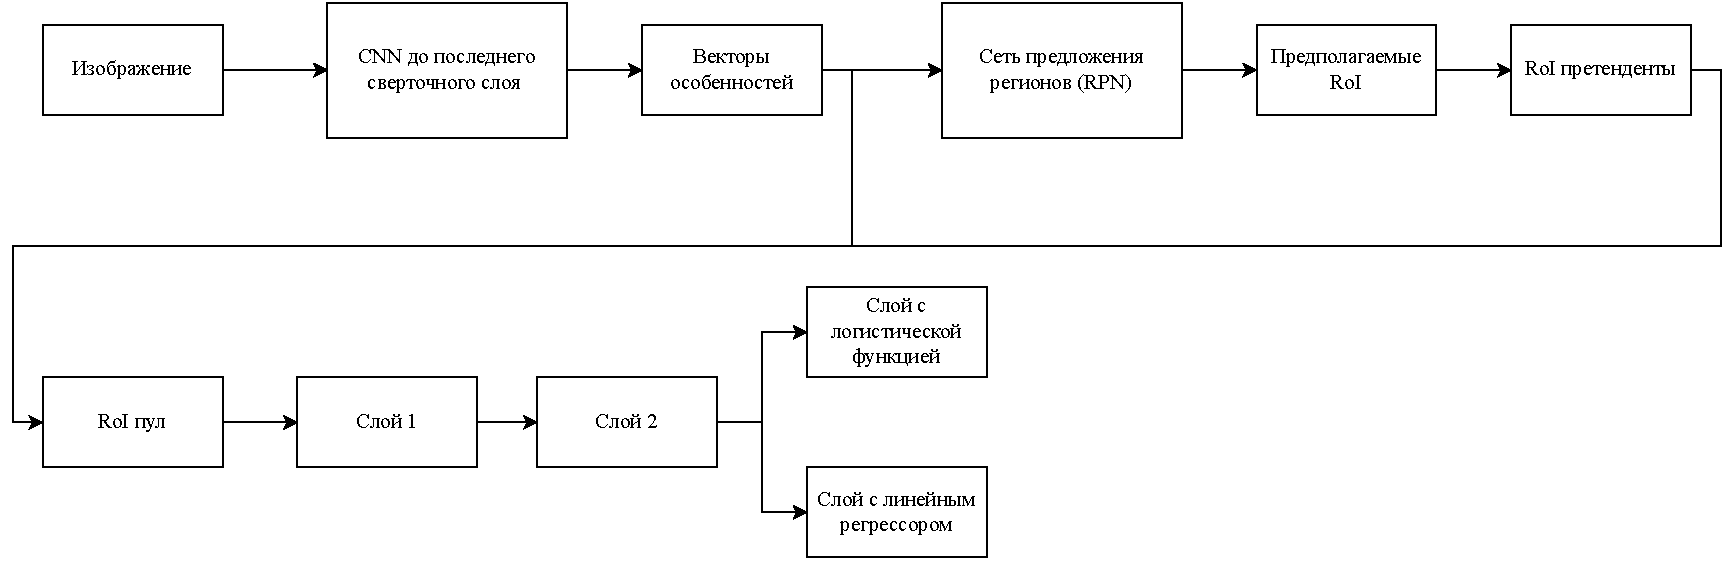
\includegraphics[width=\textwidth]{img/fasterrcnn.pdf}
	\caption{Принцип работы Faster R--CNN}
	\label{fig:fasterrcnn}
\end{figure}

Замена генерации претендентов избирательным поиском на нейронную сеть позволяет повысить быстродействие распознавания образов на изображений до десяти раз \cite{fasterrcnn}.

\subsubsection*{Вывод}
Была рассмотрена задача распознавания образов (классификации), виды классификаторов и их применимость при распознавании образов.

Было дано определение понятия нейронной сети, рассмотрены виды нейронных сетей и принцип их работы.

Были рассмотрены особенности применения нейронных сетей в качестве классификаторов.

Были рассмотрены и проанализированы технологии (R--CNN, Fast R--CNN и Faster R--CNN) для распознавания образов при помощи нейронных сетей, приведены преимущества и недостатки рассмотренных технологий.